\documentclass{beamer} % [aspectratio=169]
\usetheme{ucl}
\setbeamercolor{banner}{bg=darkred}
\setbeamersize{description width=2em}
\setbeamertemplate{navigation symbols}{\vspace{-2ex}} 
\usepackage{soul}

%\usepackage{fontspec}
\usepackage[utf8]{inputenc}
% \usepackage[english, greek]{babel}


\usepackage[T1]{fontenc} % Turn £ into $
\usepackage{minted}
\usemintedstyle{emacs}

\usepackage{fancyvrb}
\usepackage{xcolor}
\usepackage{url}

\usepackage{natbib}
\usepackage{bibentry}
\usepackage{url}
\usepackage{amsfonts}


\usepackage{tikz}
\usetikzlibrary{positioning}
\usetikzlibrary{calc,shapes.multipart,chains,arrows}
\usetikzlibrary{shapes,snakes}

\tikzset{
  treenode/.style = {align=center, inner sep=0pt, text centered,
    font=\sffamily},
  arn_n/.style = {treenode, circle, draw=black,
     text width=1.5em},% arbre rouge noir, noeud noir
  arn_r/.style = {treenode, circle, red, draw=red, 
    text width=1.5em, very thick},% arbre rouge noir, noeud rouge
  arn_d/.style = {treenode, star, star points=10, red, draw=red, 
    text width=1.5em, very thick},% arbre rouge noir, noeud rouge
  arn_x/.style = {treenode, rectangle, draw=black}% arbre rouge noir, nil
}

\newcommand\emc[1]{\textcolor{midred}{\textbf{#1}}}
\newcommand\good[1]{\textcolor{darkgreen}{\textbf{#1}}}
\newcommand\bad[1]{\textcolor{red}{\textbf{#1}}}

\AtBeginSection[]{
  \begin{frame}
  \vfill
  \centering
  \begin{beamercolorbox}[sep=8pt,center,shadow=true,rounded=true]{title}
    \usebeamerfont{title}\insertsectionhead\par%
  \end{beamercolorbox}
  \vfill
  \end{frame}
}

\author{Mark Handley, University College London, UK}
\title{Dynamic Data Structures: Trees}
\subtitle{ENGF0002: Design and Professional Skills }
% \institute{}
\date{Term 1, 2018}


\begin{document}
\nobibliography*


\frame{
\titlepage
}

\begin{frame}
  \frametitle{The story so far} %
  \begin{columns}
\begin{column}{0.5\textwidth}
  \textbf{Python lists} (aka arrays):
  \begin{itemize}
  \item \good{Fast append} to end
  \item \bad{Slow addition} anywhere other than end
  \item \bad{Slow deletion} anywhere other than end
  \item \good{Fast access} to data \textbf{by index} (ie position)
  \item \bad{Slow access} to data \textbf{by value}
  \item If we need fast access by value, can sort the data, and then do \good{binary search.}
  \end{itemize}
\end{column}
\begin{column}{0.5\textwidth}
  \textbf{Linked lists}
  \begin{itemize}
  \item \good{Fast append} to end
  \item \good{Fast addition} anywhere, if you know the \textbf{previous node}
  \item \good{Fast deletion} anywhere, if you know the \textbf{previous node}
  \item \bad{Slow access} to data \textbf{by index}
  \item \bad{Slow access} to data \textbf{by value}
  \item \bad{Can't do binary search}, even on sorted data.
  \end{itemize}
\end{column}
\end{columns}
\end{frame}

\section{Storing and retrieving data by key}

\begin{frame}
\frametitle{Motivation: keeping indexes for dynamic data structures.}

What next?
\begin{itemize}
  \item Searching is faster in sorted structures. Binary search is $\mathcal{O}(\log N)$.
  \item However, the cost of sorting is $\mathcal{O}(N \cdot \log N)$.
  \item What to do when \emc{adding or removing elements?} Sort again? No.
  \item Efficient data structures to maintain sorted sequences, and search in them
\end{itemize}

Key example: \emc{binary sorted tree}, allowing $\mathcal{O}(\log N)$ \emc{insert, remove and lookup}.


\end{frame}

\begin{frame}[fragile]
\frametitle{Trees and sorted trees.}

A tree is composed of a set of nodes. Each contains a key (and possibly a value), and links to left and right child nodes.

\begin{center}
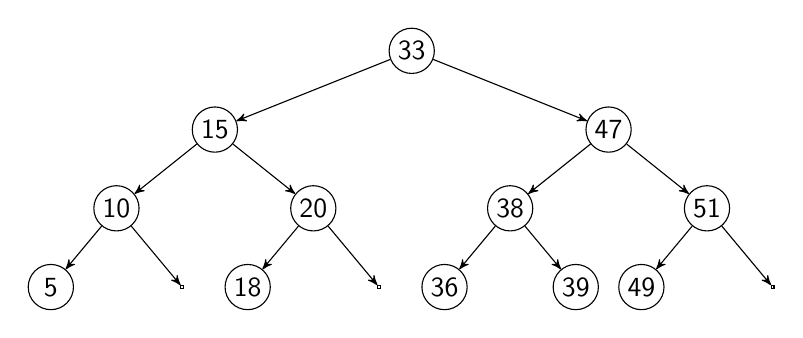
\begin{tikzpicture}[->,>=stealth',level/.style={sibling distance = 5cm/#1,
  level distance = 1cm}] 
\node [arn_n] {33}
    child{ node [arn_n] {15} 
            child{ node [arn_n] {10} 
              child{ node [arn_n] {5}} %edge from parent node[above left]
                         %{$x$}} %for a named pointer
              child{ node [arn_x] {}}
            }
            child{ node [arn_n] {20}
              child{ node [arn_n] {18}}
              child{ node [arn_x] {}}
            }                            
    }
    child{ node [arn_n] {47}
            child{ node [arn_n] {38} 
              child{ node [arn_n] {36}}
              child{ node [arn_n] {39}}
            }
            child{ node [arn_n] {51}
              child{ node [arn_n] {49}}
              child{ node [arn_x] {}}
            }
    }
; 
\end{tikzpicture}
\end{center}

\emc{Invariant} of a sorted binary tree: at every node, \emc{left child's key is less than or equal to the key of its parent}.  Similarly, the right child's key is larger.

\end{frame}

\begin{frame}
\frametitle{Representing a TreeNode as a Python class.}

Each TreeNode is an instance of a class, containing four attributes. 
\inputminted[
    firstline=1,
    lastline=6,
    xleftmargin=1.4em,
    %frame=lines,
    %framesep=2mm,
    %baselinestretch=1.2,
    bgcolor=stone,
    fontsize=\scriptsize,
    %linenos
  ]{python}{src/binaryTree.py}
By convention we represent a missing child as \texttt{None}.

We'll keep the tree sorted by \emc{key}, while \emc{value} can be any
data we wish to find quickly using the key.

\end{frame}

\begin{frame}[fragile]
\frametitle{How to add an element to the Tree.}

How to insert an item with key 25 to the tree?

\begin{center}
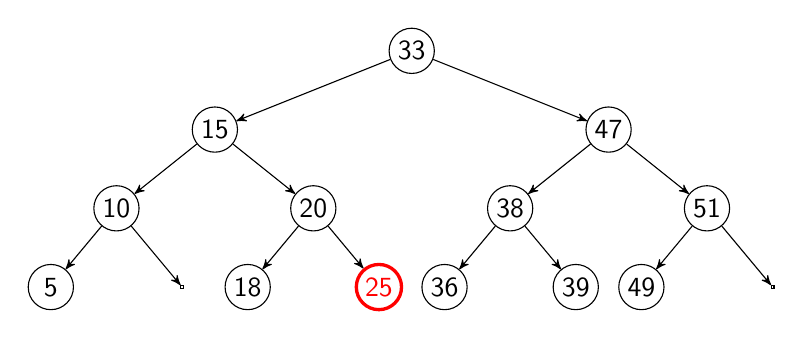
\begin{tikzpicture}[->,>=stealth',level/.style={sibling distance = 5cm/#1,
  level distance = 1cm}] 
\node [arn_n] {33}
    child{ node [arn_n] {15} 
            child{ node [arn_n] {10} 
              child{ node [arn_n] {5}} %edge from parent node[above left]
                         %{$x$}} %for a named pointer
              child{ node [arn_x] {}}
            }
            child{ node [arn_n] {20}
              child{ node [arn_n] {18}}
              child{ node [arn_r] {25}}
            }                            
    }
    child{ node [arn_n] {47}
            child{ node [arn_n] {38} 
              child{ node [arn_n] {36}}
              child{ node [arn_n] {39}}
            }
            child{ node [arn_n] {51}
              child{ node [arn_n] {49}}
              child{ node [arn_x] {}}
            }
    }
; 
\end{tikzpicture}
\end{center}
Navigate from the root of the tree to the position where the item should be inserted, at a leaf, and place a new branch there with the item.

\end{frame}

\begin{frame}
\frametitle{Adding a node}

Follow the correct left or right branch according to the invariant. When it finds the first empty leaf (\texttt{None}) insert a new branch with the item.
\inputminted[
    firstline=8,
    lastline=18,
    xleftmargin=1.4em,
    %frame=lines,
    %framesep=2mm,
    %baselinestretch=1.2,
    bgcolor=stone,
    fontsize=\footnotesize,
    %linenos
  ]{python}{src/binaryTree.py}
Note the use of recursion; and the mutation of the tree.

\end{frame}

\begin{frame}[fragile]
\frametitle{Finding an item}

How to find node with key 36?

\begin{center}
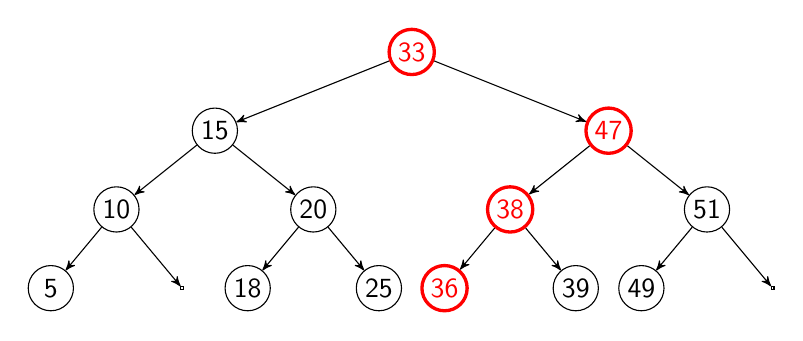
\begin{tikzpicture}[->,>=stealth',level/.style={sibling distance = 5cm/#1,
  level distance = 1cm}] 
\node [arn_r] {33}
    child{ node [arn_n] {15} 
            child{ node [arn_n] {10} 
              child{ node [arn_n] {5}} %edge from parent node[above left]
                         %{$x$}} %for a named pointer
              child{ node [arn_x] {}}
            }
            child{ node [arn_n] {20}
              child{ node [arn_n] {18}}
              child{ node [arn_n] {25}}
            }                            
    }
    child{ node [arn_r] {47}
            child{ node [arn_r] {38} 
              child{ node [arn_r] {36}}
              child{ node [arn_n] {39}}
            }
            child{ node [arn_n] {51}
              child{ node [arn_n] {49}}
              child{ node [arn_x] {}}
            }
    }
; 
\end{tikzpicture}
\end{center}
Navigate from the root of the tree, going left if the key is less than the current node's key, right if it's greater.  

\end{frame}

\begin{frame}
\frametitle{Finding items.}

A recursive \emc{divide-and-conquer} algorithm for finding a node by key.
\inputminted[
    firstline=21,
    lastline=33,
    xleftmargin=1.4em,
    %frame=lines,
    %framesep=2mm,
    %baselinestretch=1.2,
    bgcolor=stone,
    fontsize=\footnotesize,
    %linenos
  ]{python}{src/binaryTree.py}

\end{frame}

\begin{frame}
\frametitle{Hiding the internal implementation from users}

\inputminted[
    firstline=91,
    lastline=93,
    xleftmargin=1.4em,
    %frame=lines,
    %framesep=2mm,
    %baselinestretch=1.2,
    bgcolor=stone,
    fontsize=\footnotesize,
    %linenos
]{python}{src/binaryTree.py}
\vspace{-8mm}
\inputminted[
    firstline=99,
    lastline=105,
    xleftmargin=1.4em,
    %frame=lines,
    %framesep=2mm,
    %baselinestretch=1.2,
    bgcolor=stone,
    fontsize=\footnotesize,
    %linenos
  ]{python}{src/binaryTree.py}
\vspace{-8mm}
\inputminted[
    firstline=117,
    lastline=123,
    xleftmargin=1.4em,
    %frame=lines,
    %framesep=2mm,
    %baselinestretch=1.2,
    bgcolor=stone,
    fontsize=\footnotesize,
    %linenos
  ]{python}{src/binaryTree.py}

\end{frame}
\begin{frame}
\frametitle{Hiding the internal implementation from users}

Users don't want to see how a binary tree is implemented.  They just want an API that is simple to use:

\inputminted[
    firstline=201,
    lastline=206,
    xleftmargin=1.4em,
    %frame=lines,
    %framesep=2mm,
    %baselinestretch=1.2,
    bgcolor=stone,
    fontsize=\footnotesize,
    %linenos
]{python}{src/binaryTree.py}

\end{frame}

\begin{frame}[fragile]
\frametitle{Removing items --- Case 1: removing a leaf.}

When removing a leaf (node with no children, eg.\ 49) we can simply replace it with \texttt{None} in the parent.
\begin{center}
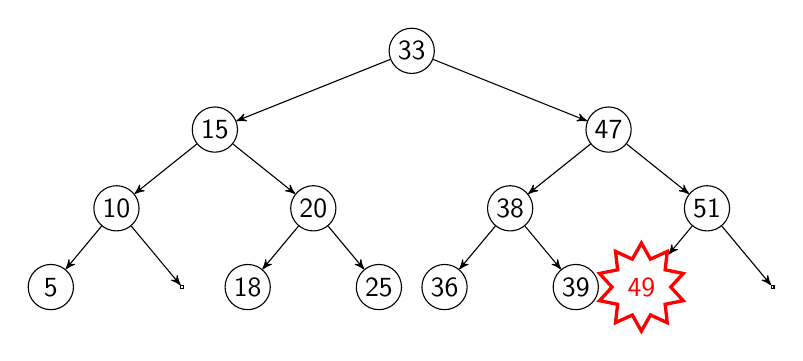
\begin{tikzpicture}[->,>=stealth',level/.style={sibling distance = 5cm/#1,
  level distance = 1cm}] 
\node [arn_n] {33}
    child{ node [arn_n] {15} 
            child{ node [arn_n] {10} 
              child{ node [arn_n] {5}} %edge from parent node[above left]
                         %{$x$}} %for a named pointer
              child{ node [arn_x] {}}
            }
            child{ node [arn_n] {20}
              child{ node [arn_n] {18}}
              child{ node [arn_n] {25}}
            }                            
    }
    child{ node [arn_n] {47}
            child{ node [arn_n] {38} 
              child{ node [arn_n] {36}}
              child{ node [arn_n] {39}}
            }
            child{ node [arn_n] {51}
              child{ node [arn_d] {49}}
              child{ node [arn_x] {}}
            }
    }
; 
\end{tikzpicture}
\end{center}
\end{frame}

\begin{frame}[fragile]
\frametitle{Case 2 \& 3: remove an incomplete branch.}

When the node to be removed has only one child (eg.\ 51), we can simply `promote up' that child. 
\begin{center}
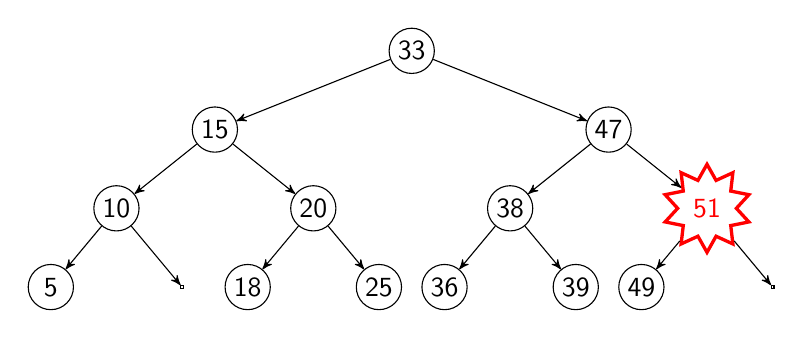
\begin{tikzpicture}[->,>=stealth',level/.style={sibling distance = 5cm/#1,
  level distance = 1cm}] 
\node [arn_n] {33}
    child{ node [arn_n] {15} 
            child{ node [arn_n] {10} 
              child{ node [arn_n] {5}} %edge from parent node[above left]
                         %{$x$}} %for a named pointer
              child{ node [arn_x] {}}
            }
            child{ node [arn_n] {20}
              child{ node [arn_n] {18}}
              child{ node [arn_n] {25}}
            }                            
    }
    child{ node [arn_n] {47}
            child{ node [arn_n] {38} 
              child{ node [arn_n] {36}}
              child{ node [arn_n] {39}}
            }
            child{ node [arn_d] {51}
              child{ node [arn_n] {49}}
              child{ node [arn_x] {}}
            }
    }
; 
\end{tikzpicture}
\end{center}

\end{frame}



\begin{frame}[fragile]
\frametitle{Case 4: a full branch}

Removing a node with two children (eg.\ 47) leaves a `hole' in the tree. We need to substitute the node with another one. A good candidate for a substitude is the node in the left subtree with the largest key (eg.\ 39).

\begin{center}
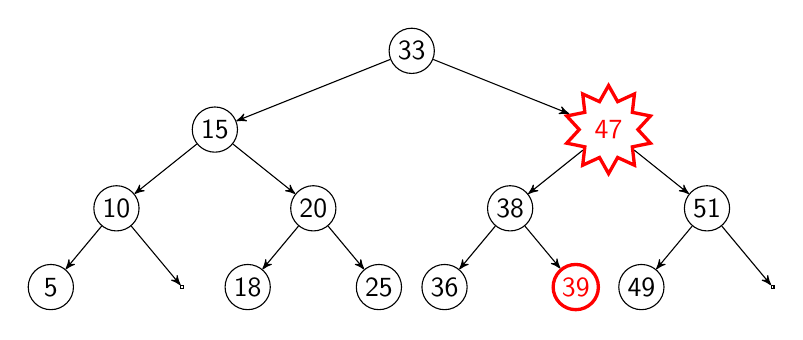
\begin{tikzpicture}[->,>=stealth',level/.style={sibling distance = 5cm/#1,
  level distance = 1cm}] 
\node [arn_n] {33}
    child{ node [arn_n] {15} 
            child{ node [arn_n] {10} 
              child{ node [arn_n] {5}} %edge from parent node[above left]
                         %{$x$}} %for a named pointer
              child{ node [arn_x] {}}
            }
            child{ node [arn_n] {20}
              child{ node [arn_n] {18}}
              child{ node [arn_n] {25}}
            }                            
    }
    child{ node [arn_d] {47}
            child{ node [arn_n] {38} 
              child{ node [arn_n] {36}}
              child{ node [arn_r] {39}}
            }
            child{ node [arn_n] {51}
              child{ node [arn_n] {49}}
              child{ node [arn_x] {}}
            }
    }
; 
\end{tikzpicture}
\end{center}

\end{frame}

\begin{frame}
\frametitle{The remove API}

\inputminted[
    firstline=193,
    lastline=203,
    xleftmargin=1.4em,
    %frame=lines,
    %framesep=2mm,
    %baselinestretch=1.2,
    bgcolor=stone,
    fontsize=\scriptsize,
    %linenos
  ]{python}{src/binaryTree.py}


\end{frame}

\begin{frame}
\frametitle{The BinaryTree implementation}

\inputminted[
    firstline=91,
    lastline=93,
    xleftmargin=1.4em,
    %frame=lines,
    %framesep=2mm,
    %baselinestretch=1.2,
    bgcolor=stone,
    fontsize=\footnotesize,
    %linenos
]{python}{src/binaryTree.py}
\inputminted[
    firstline=109,
    lastline=112,
    xleftmargin=1.4em,
    %frame=lines,
    %framesep=2mm,
    %baselinestretch=1.2,
    bgcolor=stone,
    fontsize=\scriptsize,
    %linenos
  ]{python}{src/binaryTree.py}

Almost all the work happens in the TreeNode's \texttt{delete()} method.

\end{frame}

\begin{frame}
\frametitle{TreeNode's delete() implementation.}

\inputminted[
    firstline=50,
    lastline=70,
    xleftmargin=1.4em,
    %frame=lines,
    %framesep=2mm,
    %baselinestretch=1.2,
    bgcolor=stone,
    fontsize=\scriptsize,
    %linenos
  ]{python}{src/binaryTree-slideware.py}


\end{frame}

\begin{frame}
%\frametitle{Traversing in order: Depth-first traversal}

\textbf{Depth-first traversal} involves returning items, by first returning all nodes in the left branch, then the item, and all items in the right branch. As the tree is sorted, items are returned in order.

\vspace{2mm}
In BinaryTree class:
\vspace{-3mm}
\inputminted[
    firstline=126,
    lastline=129,
    xleftmargin=1.4em,
    %baselinestretch=1.2,
    bgcolor=stone,
    fontsize=\scriptsize,
    %linenos
  ]{python}{src/binaryTree.py}

\vspace{-5mm}
In TreeNode class:
\vspace{-3mm}
\inputminted[
    firstline=83,
    lastline=88,
    xleftmargin=1.4em,
    %baselinestretch=1.2,
    bgcolor=stone,
    fontsize=\scriptsize,
    %linenos
  ]{python}{src/binaryTree.py}

\vspace{-5mm}
This is a \emc{generator} defined through keyword \texttt{yield}. The keyword \texttt{yield from} returns items from another generator until it's \emc{exhausted}, then continues the execution. See \texttt{\scriptsize https://wiki.python.org/moin/Generators}.

\end{frame}

\begin{frame}
\frametitle{Testing add and remove}

We test at the level of the interface, not internal representation.
\inputminted[
    firstline=222,
    lastline=239,
    xleftmargin=1.4em,
    %baselinestretch=1.2,
    bgcolor=stone,
    fontsize=\scriptsize,
    %%linenos
  ]{python}{src/binaryTree-slideware.py}

\end{frame}

\begin{frame}
\frametitle{Testing the iterator}

We ensure that iterating returns elements in order.
\inputminted[
    firstline=242,
    lastline=258,
    xleftmargin=1.4em,
    %baselinestretch=1.2,
    bgcolor=stone,
    fontsize=\scriptsize,
    %%linenos
  ]{python}{src/binaryTree-slideware.py}

\end{frame}


\begin{frame}
\frametitle{Computational complexity.}

Average case operation:
\begin{itemize}
  \item \emc{add}, \emc{remove}, \emc{get}: $\mathcal{O}(\log N)$
  \item \emc{walk} walks the full tree: $\mathcal{O}(N)$
\end{itemize}

\vspace{3mm}
\begin{block}{Advanced data structures: Balanced trees}
The average case performance is only attained if the tree is `balanced'. However trees might get unbalanced under dynamic additions and deletions (consider adding elements in order). Balanced binary trees are needed to ensure balance is maintained for $\mathcal{O}(\log N)$ operations.
\end{block}

\end{frame}

\begin{frame}
\frametitle{The builtin \texttt{dict} type.}

The Python dictionary type provides a very efficient key-value store.
\begin{itemize}
  \item the \texttt{dict} function takes a sequence of tuples and returns a dictionary mapping them as key values.
  \item There is a shorthand for dict literals, eg. \texttt{\{k1:v1, k2:v2\}}
  \item Get and set operations are as in minimap, eg. \texttt{m[k] = v} for set, and \texttt{m[k]} for get.
  \item the \texttt{len} function returns the number of items, and an iterator returns an unordered sequence of keys.
\end{itemize}

\vspace{3mm} 
For a full list of operations see \url{https://docs.python.org/3.7/library/stdtypes.html\#mapping-types-dict}.
\end{frame}

\bibliographystyle{alpha}
\nobibliography{references}

\end{document}
